\subsection{Mobile App}
Die Mobile App dient einerseits als Interaktionsschnittstelle zwischen Nutzer und Sprachassistent und andererseits als Konfigurator der Privatsphäre. Die App bietet folgende vier Ansichten:

\begin{itemize}
    \item Registrierung: Ein neuer Nutzer kann sich mit seiner E-Mail und einem Passwort beim Sprachassistenten registrieren. Dabei kann der Nutzer zwischen den Profiltypen Privat, Arzt oder Mobilitätsunterstützung auswählen. Je nach Profiltyp werden unterschiedliche Privatsphäre-Einstellungen vorkonfiguriert. Standardmäßig ist ein privates Profil nur für den Besitzer zugänglich, wohingegen die Profiltypen Arzt und Mobilitätsunterstützung öffentlich zugänglich sind. 
    \item Login: Ein registrierter Nutzer kann sich mit seiner E-Mail und seinem Passwort bei dem Sprachassistenten anmelden.
    \item Sprachassistent: Der Sprachassistent ist die Hauptansicht der App, welche erscheint, sobald ein Nutzer eingeloggt ist. Gleichzeitig wird auch die Hotword Detection gestartet, welche mit Snowboy von Kitt.au realisiert wurde \cite{SnowboyHotwordDetection}. Die Hotword Detection lauscht lokal auf dem Smartphone, bis das Signalwort \glqq Butler\grqq{} erkannt wird, dabei werden keine Daten gespeichert und an Dritte weitergegeben. Nachdem Erkennen des Signalwortes wird die Sprachverarbeitung aufgrund besserer Performance in die Cloud verlagert. Sobald eine Interaktion zwischen Nutzer und Sprachassistent beendet ist, wird die Hotword Detection wieder aktiviert. Des Weiteren werden alle Ausgaben des Sprachassistenten auf der Ansicht ausgegeben. Die Audioaufnahme und Wiedergabe wurde mit der Android \acrshort{sdk} umgesetzt.
    \item Einstellungen: Diese Ansicht bietet dem Nutzer die Möglichkeit, sein Profil und Privatsphäre-Einstellungen zu konfigurieren. Für das Profil kann der Vor- und Nachname festgelegt werden. Der Standort kann entweder per Texteingabe oder per GPS ermittelt werden. Bei der Ermittlung des Standortes per GPS kann der Nutzer entscheiden, ob der Standort einmalig abgerufen wird oder die App automatisch diesen aktualisiert. Der Nutzer kann seinen Kalender der App zur Verfügung stellen. Dabei kann zusätzlich das automatische Aktualisieren des Kalenders oder das Verstecken von Details, wie Titel und Beschreibung eines Termins, aktiviert werden. Somit wird nur Zugriff auf die für den Anwendungsfall relevante Daten gewährleistet. Andere personenbezogene Daten, wie Name des Kalenders oder des Besitzers kann die App nicht ermitteln. Als Nächstes kann der Nutzer Mobilitätsunterstützungen festlegen, die beim Zustande kommen eines Termins mit einem Arzt standardmäßig angefordert werden. Dabei kann einerseits Scala Mobile, welches dem Nutzer beim Verlassen des Hauses hilft, oder anderseits ein Abholservice, der den Nutzer zum Arzt befördert, angefordert werden. Das Profil sowie die Privatsphäre-Einstellungen werden mit dem Privacy Provider synchronisiert. Durch diese App-Ansicht kann die im Konzept vorgestellte Datensparsamkeit  sowie die Nutzergesteuerte Privatsphäre ermöglicht werden.
\end{itemize}

\begin{figure}[!ht]
	\centering
	\begin{subfigure}[t]{0.48\linewidth}
		\centering
		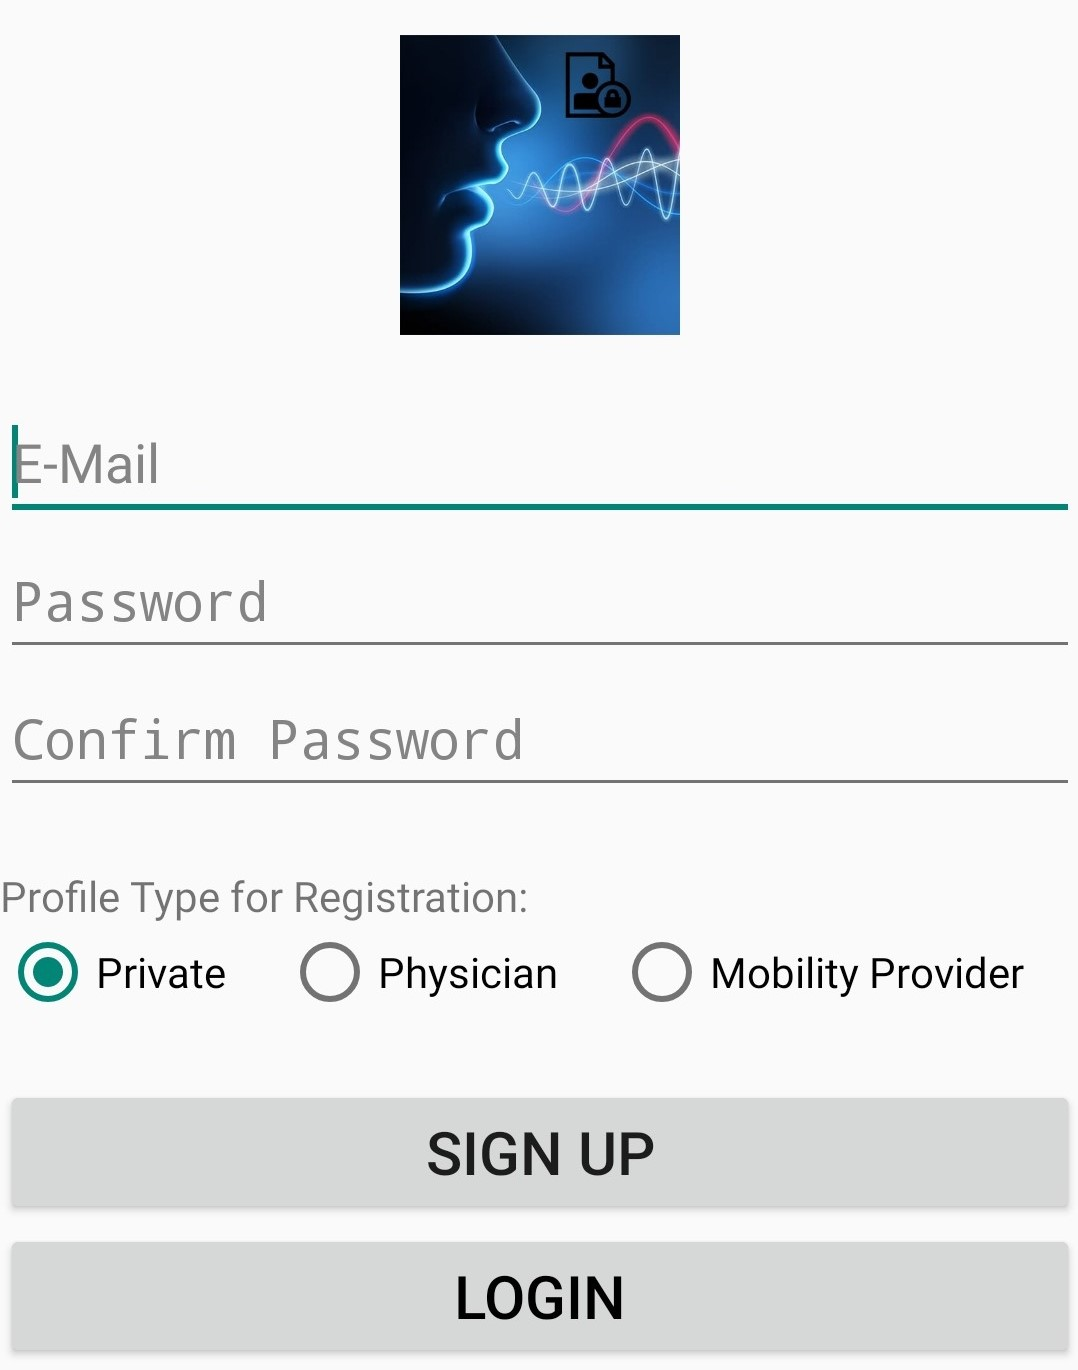
\includegraphics[width=1\linewidth]{Picture/MobileApp_Screenshot-2}
		\caption{Registrierungs-Ansicht}
		\label{fig:prototyp2}
	\end{subfigure}
	\bigskip 
	\begin{subfigure}[t]{0.48\linewidth}
		\centering
		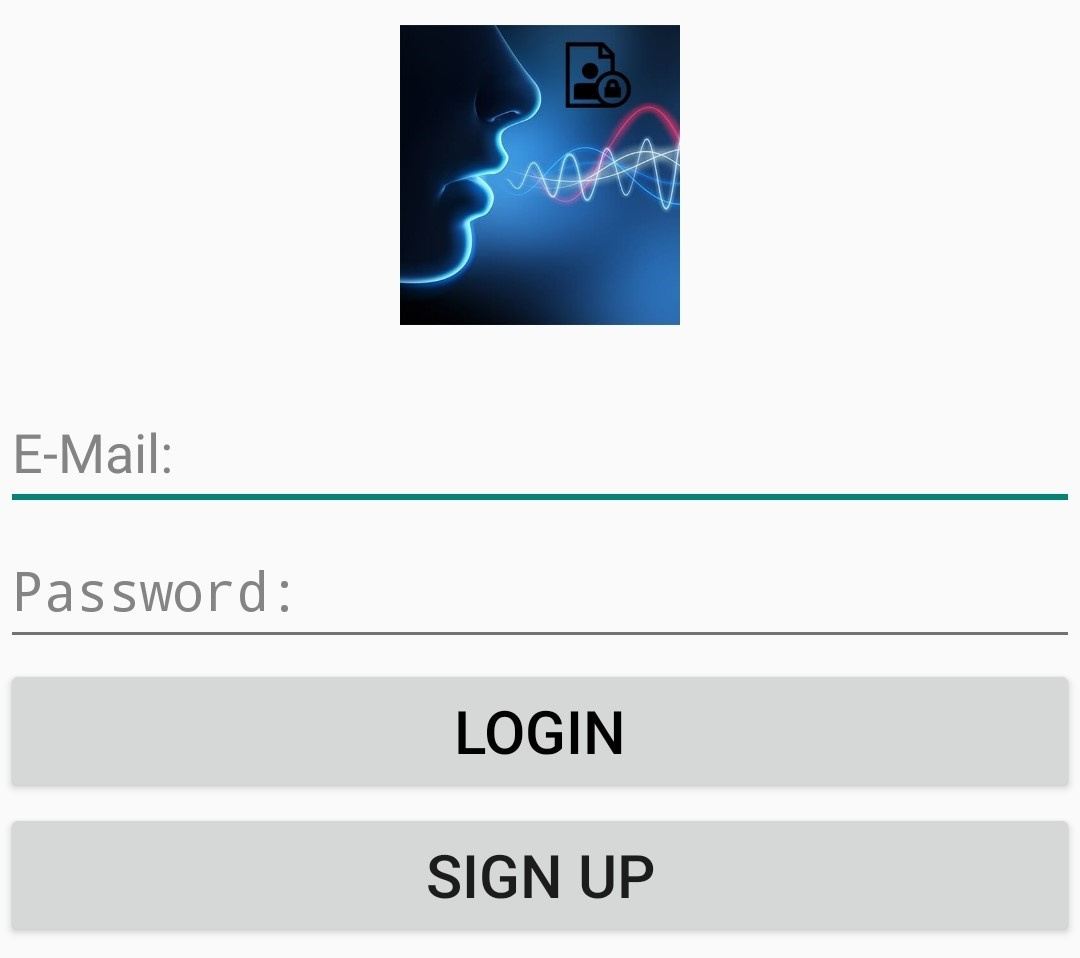
\includegraphics[width=1\linewidth]{Picture/MobileApp_Screenshot-1}
		\caption{Login-Ansicht}
		\label{fig:prototyp1}
	\end{subfigure}
	\bigskip 
	\begin{subfigure}[t]{0.48\linewidth}
		\centering
		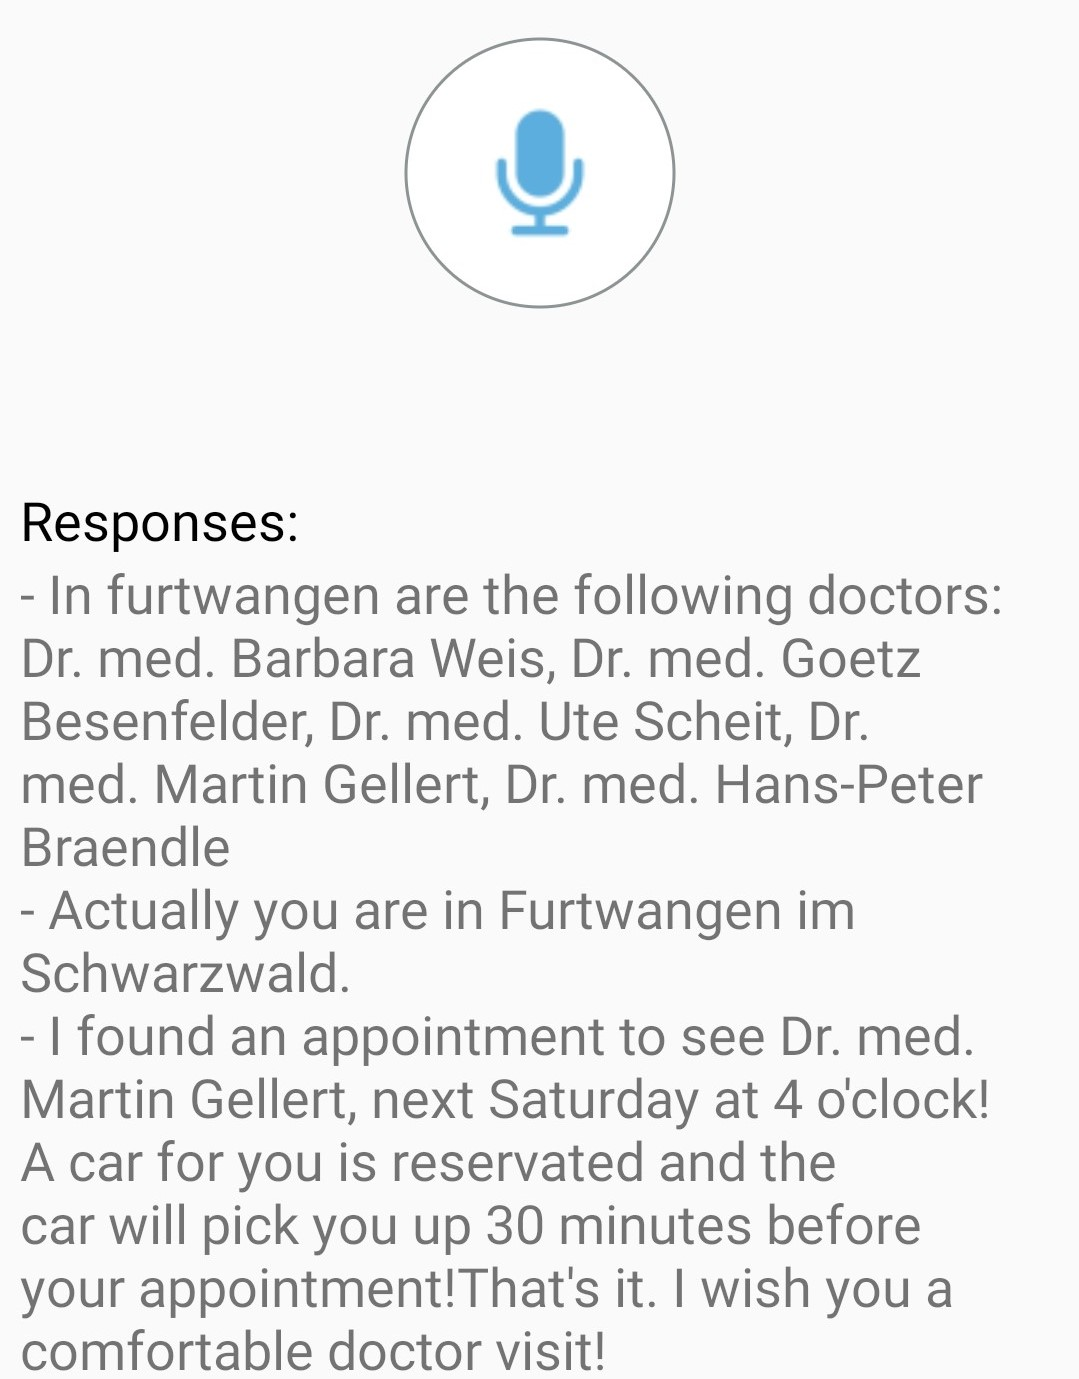
\includegraphics[width=1\linewidth]{Picture/MobileApp_Screenshot-3}
		\caption{Sprachassistent-Ansicht}
		\label{fig:prototyp3}
	\end{subfigure}
	\begin{subfigure}[t]{0.48\linewidth}
		\centering
		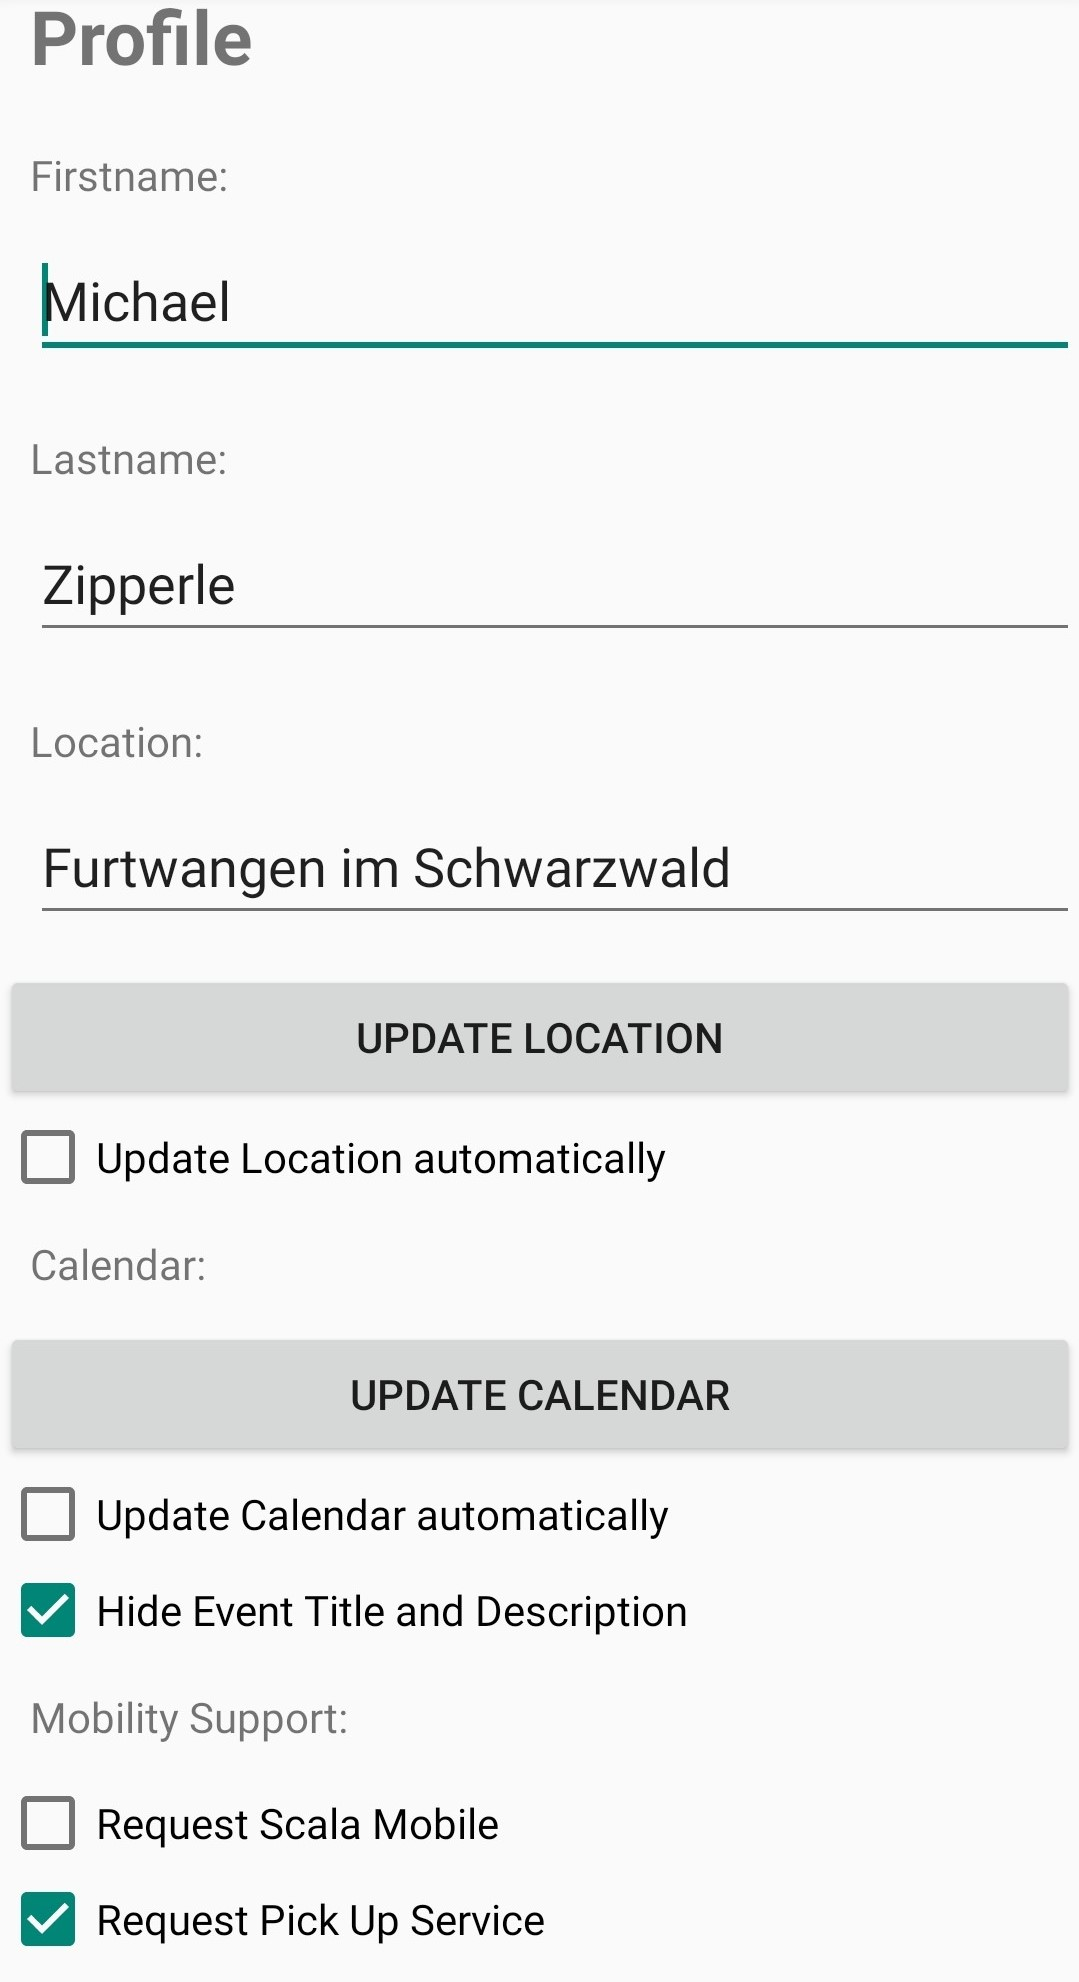
\includegraphics[width=1\linewidth]{Picture/MobileApp_Screenshot-4}
		\caption{Einstellungen-Ansicht}
		\label{fig:prototyp3}
	\end{subfigure}
	\caption{Mobile App}
	\label{fig:mobileapp}
\end{figure}